\documentclass[12pt, a4paper]{article}

\usepackage{amsmath}
\usepackage{bm}
\usepackage{array}
\usepackage{amsmath}
\usepackage[portuguese]{babel}
\usepackage{chngpage}
\usepackage{float}
\usepackage[a4paper, margin=2cm]{geometry}
\usepackage{graphicx}
\usepackage{hyperref}
\usepackage{listings}
\usepackage{setspace}
\usepackage{xcolor}

\lstdefinestyle{codestyle}{
    commentstyle=\color{teal},
    keywordstyle=\color{blue},
    numberstyle=\ttfamily\color{gray},
    stringstyle=\color{red},
    basicstyle=\ttfamily\footnotesize,
    breakatwhitespace=false,
    breaklines=false,
    keepspaces=true,
    numbers=none,
    showspaces=false,
    showstringspaces=false,
    showtabs=false,
    tabsize=4
}
\lstset{style=codestyle}

\title{\Huge \textbf{Computação Gráfica \\ \Large Trabalho Prático -- Fase IV}}
\date{18 de maio de 2025}
\author{Grupo 3}

\begin{document}

\begin{center}
    
\includegraphics[width=0.25\textwidth]{res/cover/EE-C.eps}
\end{center}

\chardef\_=`_
\onehalfspacing
\setlength{\parskip}{\baselineskip}
\setlength{\parindent}{0pt}
\def\arraystretch{1.5}

{\let\newpage\relax\maketitle}
\maketitle
\thispagestyle{empty}

\vspace*{\fill}

\begin{adjustwidth}{-2cm}{-2cm} % These values only need to be large enough to center the table
    \begin{center}
        \begin{tabular}{>{\centering}p{0.25\textwidth}
                        >{\centering}p{0.25\textwidth}
                        >{\centering}p{0.25\textwidth}
                        >{\centering\arraybackslash}p{0.25\textwidth}}
            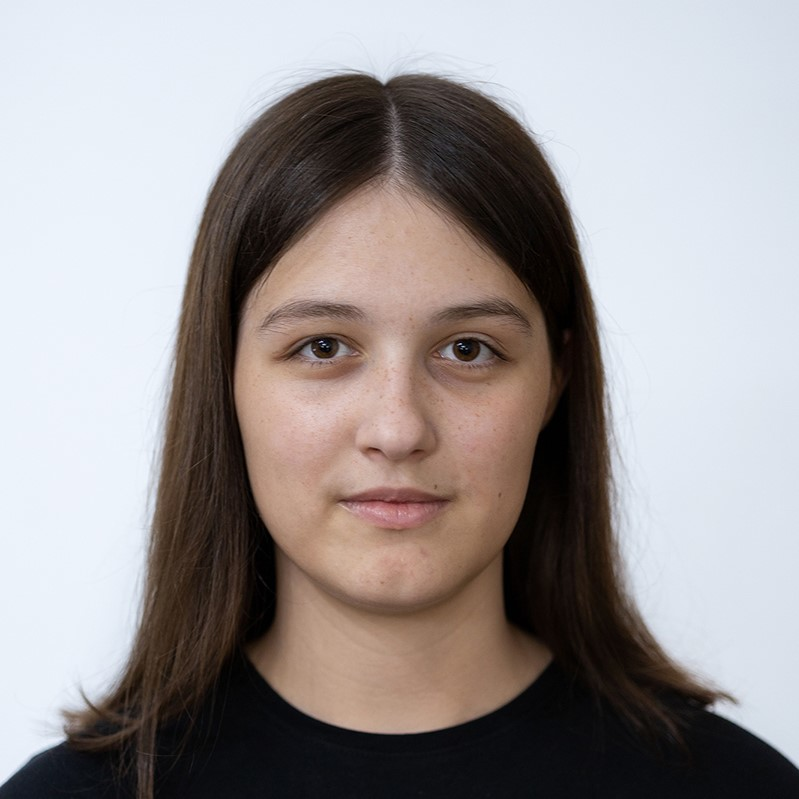
\includegraphics[width=3.5cm]{res/cover/A104437.png} &
            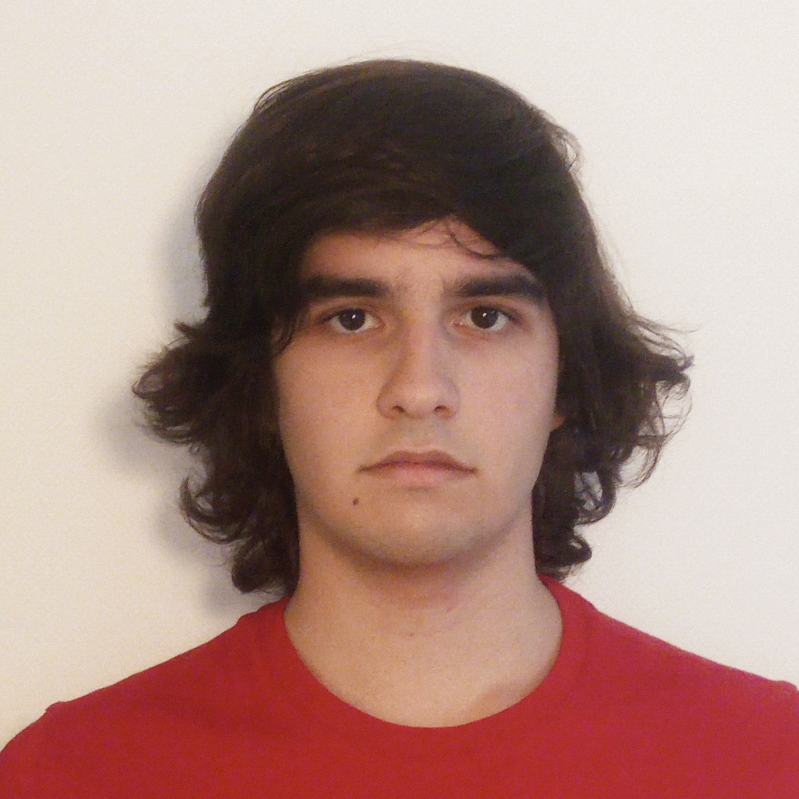
\includegraphics[width=3.5cm]{res/cover/A104348.png} &
            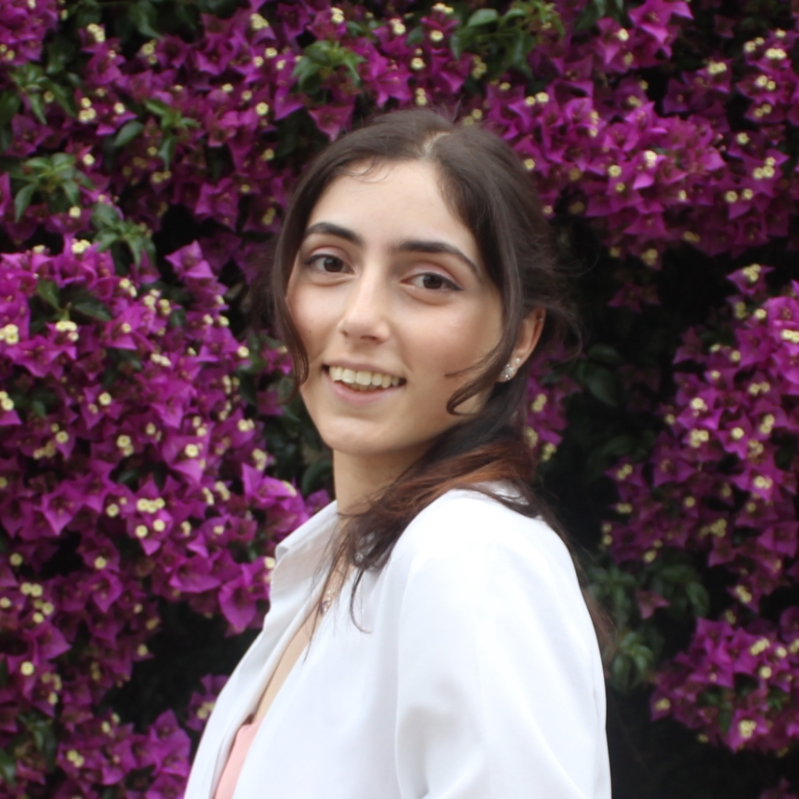
\includegraphics[width=3.5cm]{res/cover/A90817.png} &
            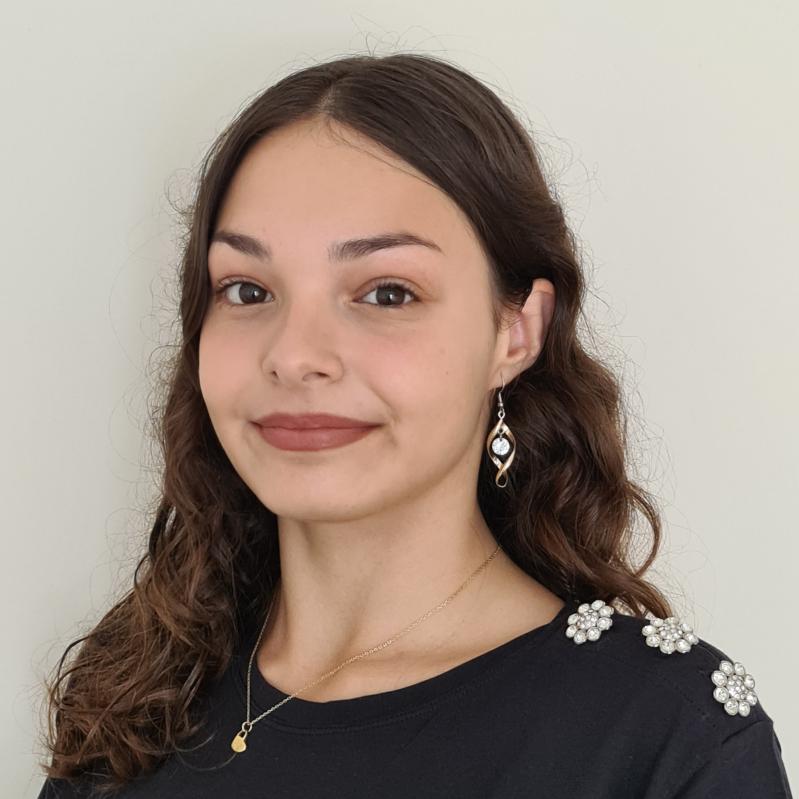
\includegraphics[width=3.5cm]{res/cover/A104179.png} \\

            Ana Oliveira & Humberto Gomes & Mariana Cristino & Sara Lopes \\
            A104437      & A104348        & A90817           & A104179
        \end{tabular}
    \end{center}
\end{adjustwidth}

\pagebreak

\begin{abstract}
    \noindent
    {\color{red} TODO - Humberto}
\end{abstract}

\section{\emph{Generator}}

\subsection{Formato \texttt{.3d}}

{\color{red} TODO - Humberto}

\subsection{Plano Horizontal}

{\color{red} TODO - Humberto}

\subsection{Cubo}

{\color{red} TODO - Humberto}

\subsection{Esfera}

{\color{red} TODO - Mariana}

\subsection{Cone}

{\color{red} TODO - Ana}

\subsection{Cilindro}

{\color{red} TODO - Mariana}

\subsection{\emph{Torus}}

{\color{red} TODO - Sara}

\subsection{Outras Figuras}

{\color{red} TODO - Humberto}

\subsection{Sistema Solar}

{\color{red} TODO - Ana}

\section{\emph{Engine}}

\subsection{Geração Automática de Normais}

{\color{red} TODO - Humberto}

\subsection{Adição ao \emph{Schema} XML}

{\color{red} TODO - Mariana}

\subsection{Texturas e Normais}

{\color{red} TODO - Humberto}

\subsection{\emph{Object Picking}}

{\color{red} TODO - Sara}

\section{Resultados Obtidos}

{\color{red} TODO - cada faz as suas prints, sem borda de janela, no tamanho especificado pela cena,
com a UI escondida (U), Humberto escreve}

\section{Conclusão}

{\color{red} TODO - Humberto}

\begingroup
\section{Bibliografia}
\renewcommand{\section}[2]{}

\begin{thebibliography}{9}
\end{thebibliography}
\endgroup

\end{document}
